\chapter{XQuery/XPath 3.* Test Suite(QT3TS)}
\section{Analysis}
In this chapter, we will discuss design decisions that we have made during the development of Test Driver. The core idea is to develop Test Driver completely independently from Rumble by maintaining the code outside of Rumble.

\subsection{Programming Language}
 We view Rumble as black-box and the single point of communication with Rumble should only be via the Rumble Java public API. Therefore, we have decided to implement Test Driver as Java Console Application. Furthermore, Rumble is also written in Java. We decided to setup our Java Console Application project to have two modules - Test Driver and Rumble module. Rumble module is the branch in repository created for the purpose of this work \cite{RumbleBranch}. Making Test Driver module dependent on it, we are allowing possibility to directly use Rumble and its classes in case that not everything is possible to be achieved by treating Rumble as the black-box. 

\subsection{Data Format}
The XQuery/XPath 3.* Test Suite (QT3TS) is publicly available at W3C Public CVS Repository under module name 2011/QT3-test-suite \cite{TestSuiteCVSRepository}. Since April 1st 2019, CVS tree has been discontinued and the repository has been migrated to W3C Public GitHub repository \cite{TestSuiteGitHubRepository}. The tests are published as a set of files - test sets containing in total more than 30000 test cases. The tests are published as a set of files, mostly in XML format. W3C does not supply a Test Driver for executing the tests. Instead, for each implementation a Test Driver should be written. As these test sets are mostly written in XML format, the first component that our Test Driver will require is the XML parser. 

\subsection{XML Parser}
XML parser is a program that allows our application to read and write XML documents. For our work, we have investigated following possibilities:
\begin{itemize}
	\item DOM (Document Object Model) - This parser loads entire XML document in memory and uses interfaces to access the information. It can access couple of item elements at same time. It can be used for both reading and writing.
	\item SAX (Simple API for XML parsing) - This parser doesn't load XML document in memory. Instead, it allows us to register a handler with SAX parser. When parser goes through file it keeps invoking methods on the handler class for each item. It process it in sequence one at a time. For each new item it reads, it forgets state of previous items. Therefore, on each read we need to take appropriate action in our application. It is read only and also known as push parser. There is no handler on XML document side, only in our application.
	\item STAX (Streaming API for XML parsing) - This parser allows us to both read and write multiple documents at same time. Unlike SAX that reads one item at a time, STAX can be explicitly asked to get a certain item from XML document without loading it in memory. Therefore, we can look at it as mixture of DOM and SAX. It is pull parser and has handler on XML document as well
	\item JAXP (JAVA API for XML parsing) - Since JDK 1.5, the JAXP API has been available as a standard part of the Java platform, and it provides access to XSLT transformation, schema validation, and XPath processing services.
	\item Saxon \cite{Saxon} - Open Source XSLT \& XQuery processor developed by Saxonica Limited. The Saxon package is a collection of tools for processing XML documents. The main components accessible via API are:
	\begin{enumerate}
		\item XSLT processor. Saxon implements the XSLT 3.0 Recommendation. The product can also be used to run XSLT 2.0 stylesheets, or XSLT 1.0 stylesheets in backwards compatibility mode.
		\item XPath processor. This supports XPath 2.0 and XPath 3.1. It can also be used in backwards-compatibility mode to evaluate XPath 1.0 expressions.
		\item XQuery processor. This supports XQuery 3.1, which also allows XQuery 1.0 or 3.0 queries to be executed. 
		\item XML Schema Processor. This supports both XSD 1.0 and XSD 1.1. It can be used to support the schema-aware functionality of the XSLT and XQuery processors.
	\end{enumerate}
\end{itemize}

For parsing XML, we have decided to use Saxon. One may argue that for all 4 listed components, Java also has its own API – JAXP for 1st, 2nd and 4th together with XQJ for 3rd. However, in practice, Saxon is easier to use and more flexible than JAXP. Apart from that, main arguments are:
\begin{enumerate}
	\item Saxon itself is one of the implementations for which Test Driver was also implemented. Based on Results Report \cite{SaxonReport}, it passes more than 99,9\% of the QT3TS tests.
	\item Saxons implementation of the Test Driver can be used as a baseline for developing our own Test Driver. 
\end{enumerate}

\section{Phase 1 Implementation}
\subsection{Description}
\label{Phase1_Description}
In the first phase of the implementation we have analyzed the structure of QT3TS. We had to understand the under-laying structure of each and every test case. We had to see under which tags the information is stored in order to obtain it using Saxon API. Example test case in XML format:

\lstinputlisting{source_code_1.xml}

The two most important tags in each test case are:
\begin{itemize}
	\item Test  - this is the test that should be executed on Rumble. It can be XSLT, XPath or XQuery expression.
	\item Result - this is the expected result outcome of the test tag. As it can be seen in the provided example, there are several types of assertions that we need to verify.
\end{itemize}

Test Driver's Test Case Handling Logic is supposed to iterate over catalog.xml using the Saxon API. This XML document contains list of all test-sets. Again, using the Saxon API, we iterate over test-cases in each of the test-sets. For each test-case, we are asking explicitly Saxon XML parser to get items under Test and Result tags. To use Saxon API, we need to know the structure. But, once Test Case Handling Logic obtains information under Test tag, it passes it down "as is" to Rumble API in order to execute the query. Rumble API returns the result which is then passed down to Test Result Handling Logic. 

Test Driver's Test Result Handling Logic is in charge of determining which assertion needs to be performed. Here we provide the list of possible assertions:

\begin{itemize}
	\item assert-empty - This assertion requires result to return empty sequence
	\item assert - This assertion requires us to run another query in which obtained result will be used as parameter of the new query. For example:
	\lstinputlisting{source_code_2.xml}
	\item assert-eq - It requires us to run another query in form of obtained result "eq" value under the assert-eq tag
	\item assert-deep-eq - Similar to assert-eq but runs "deep-equal" query
	\item assert-true - It requires result to return single Boolean value True
	\item assert-false - Opposite of assert-true
	\item assert-string-value - It requires that each item in the obtained result sequence is type of String and also "eq" to the sequence under this tag
	\item all-of - It contains multiple different assert tags described in this list and it requires all of them to be fulfilled 
	\item any-of - Similar to all-of but requires only one of them to be fulfilled
	\item assert-type - Requires to check if obtained result is instance of this tag
	\item assert-count - It requires obtained result sequence size to be equal to the value under assert-count tag
	\item not - It requires to execute nested assertion with a negation
\end{itemize}

After the assertion is performed, we need to classify the results. The idea is to make statistics that are described in \ref{Phase1_Results}. With such a classification we would be able to improve Rumble by reporting bugs in its implementation.

\subsection{Architecture}
The overview of scenario described in \ref{Phase1_Description} can be seen in Figure \ref{fig:Phase1_Architecture}
 \begin{figure}[h!]
 	\vspace*{-5mm}
 	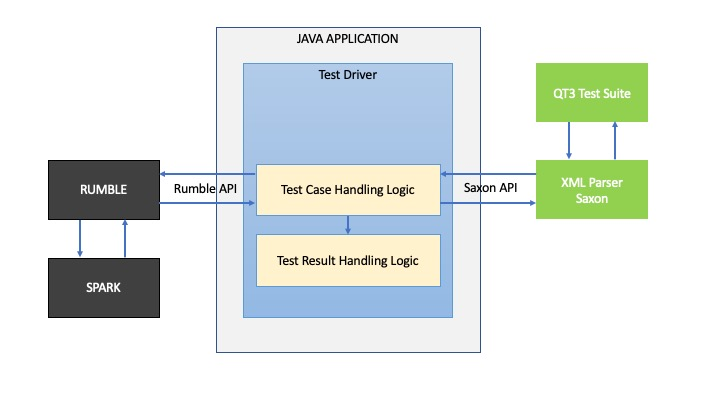
\includegraphics[width=\linewidth]{architecture_diagram_phase_1.jpeg}
 	\vspace*{-15mm}
 	\caption{Phase 1 Architecture Overview}
 	\label{fig:Phase1_Architecture}
 \end{figure}
 
\subsection{Results}

\label{Phase1_Results}
As explained in \ref{Phase1_Description}, result obtained via Rumble API was compared with the expected result by applying the correct assertion check. In case assertion passed, test-case was considered a Success and otherwise Fail. The block of code performing these operations was surrounded by try and catch. In case that test failed because the syntax was not completely JSONiq, it would throw a RumbleException or more generally an Exception - Crash. With this implementation, we were to be able to distinguish 3 possible scenarios:

\begin{enumerate}
	\item Success - Test case succeed
	\item Fail - Test case failed because of bug in Rumble
	\item Crash - Test case failed because it is not compatible with Rumble
\end{enumerate}

The report is generated as .csv file having test-sets as rows and total number of test-cases per scenario in the columns. In Table \ref{tab:Phase1_ResultTable} we will present the aggregated sum over all rows in the .csv file:

\begin{table}[h!]
	\centering
	\begin{tabular}{|l|r|r|}
		\hline
		\multicolumn{1}{|c|}{Scenario} & \multicolumn{1}{c|}{Total test-cases} & \multicolumn{1}{c|}{\% of all test-cases} \\ \hline
		Success                        & 2330                                  & 7.8                                       \\ \hline
		Fail                           & 2769                                  & 8.8                                       \\ \hline
		Crash                          & 26421                                 & 83.4                                      \\ \hline
	\end{tabular}
 	\caption{Phase 1 Results Overview}
 	\label{tab:Phase1_ResultTable}
\end{table}

\section{Phase 2 Implementation}
\subsection{Description}
\label{Phase2_Description}
After generating Phase 1 Implementation report described in Table \ref{tab:Phase1_ResultTable}, we carefully examined our implementation and identified 4 major pain points:
\begin{itemize}
	\item Unstable implementation of assertion which resulted in implementing proper way of result binding in Rumble
	\item Too many crashing tests which resulted in implementing converter
	\item Insufficient granularity for distinguishing test-cases
	\item Improving Test Driver implementation resulted in breaking previously implemented features. Therefore, regression tests were introduced
\end{itemize}

\subsubsection{Result Binding}
To better understand the issues we have encountered, we will provide following code snippet:
\lstinputlisting{source_code_without_results.java}

If we examine the AssertEq implementation, we will notice that lines.get(0) assumes that obtained result is a single item and takes first one. It does not handle sequences! Furthermore, handling sequences was only possible for AssertStringEqual in case that our result is sequence of strings by performing string concatenation. All other assertions such as Assert, AssertEq, AssertDeepEq are not possible to be implemented. Finally, if we remember Assert example from Section \ref{Phase1_Description}, we will notice that we had to perform string replace of \$result with actual result obtained from the Rumble API. 

Thus, Rumble was extended to support result binding. The change was made in Rumble implementation itself. The only modification it required was to instantiate a new RumbleConfiguration and also new Rumble instance for each test-case that requires result binding. Check code snippet below:

\lstinputlisting{source_code_with_results.java}

The main concern of the new implementation was that performing many instantiates might cause the execution time to increase dramatically. However, after run-time increased only by 15seconds from 2minutes - only 12.5\%.

Once the result binding was implemented, it allowed us to run the assert type also as a query instead of calling the publicly exposed methods of the Item class in the Rumble Java API. In Phase 1 implementation, we had a switch case for every possible type that Rumble Java API supports, making code difficult for future maintenance and extension with new supported types. With running assert type as "instance of" query , we managed to have a single point of conversion performed in the beginning and applied for both test case and the expected result. Within conversion we would discover the unsupported type errors without the need of second switch case to check whether Rumble's API Item class supports the type or not. Furthermore, the previously implemented switch case had unsupported type as default therefore hiding some types that were supported but not specified in the documentation. The mentioned conversion will be explained more in detail in Section \ref{Phase2_Converter}. 

The clean separation that was performed here initialized idea and was a base plan for XQuery to JSONiq conversion logic separation. In Section \ref{Phase3_Description} we will describe Architecture that has separate application that takes XQuery as input, performs conversion and outputs JSONiq test suite. Such approach would make the Test Driver easily maintainable and extensible!

\subsubsection{Converter}
\label{Phase2_Converter}
As seen in Table \ref{tab:Phase1_ResultTable}, we had less than 10\% Success test-cases as almost all of them required conversion to JSONiq. Here we will document all the conversions that we have performed on both Test and Result tags in this Phase. 

The first conversion that we have performed is between types. Both XQuery and JSONiq have simple(atomic) and complex(non-atomic) types. 

The list of atomic types that is currently supported by Rumble was taken from official Rumble documentation \cite{RumbleSupportedTypes} and conversion was implemented accordingly. For all types that are not supported, our code throws UnsupportedTypeException. 

Following 3 complex (non-atomic) types were handled by following conversion:
\begin{enumerate}
	\item array(*) was replaced with array*
	\item item() was replaced with item
	\item map(string, atomic) was replaced with object 
\end{enumerate}

On the other hand, following 7 complex (non-atomic) types could not be converted and they all throw UnsupportedTypeException:
\begin{enumerate}
	\item document
	\item element
	\item attribute
	\item text
	\item comment
	\item processing-instruction
	\item xs:QName
\end{enumerate}

Other conversions that were performed:
\begin{enumerate}
	\item true() was replaced with true
	\item false() was replaced with false
	\item INF was replaced with Infinity
	\item array access via . was replaced with \$\$
	\item ' was replaced with "
	\item prefixes fn, math, map, array were removed
\end{enumerate}

Other items that were unsupported in Phase 2 were node(), empty-sequence() and xs:NOTATION together with all error codes that are not in Table \ref{tab:Phase2_Supported Types} that was taken from \cite{RumbleSupportedErrorCodes}.

\begin{table}[]
	\begin{tabular}{lllr}
		\textbf{Type}      & \textbf{Status} &  & \multicolumn{1}{c}{\textbf{Supported Error Codes}} \\
		atomic             & supported       &  & FOAR0001                                           \\
		anyURI             & supported       &  & FOCA0002                                           \\
		base64Binary       & supported       &  & FODC0002                                           \\
		boolean            & supported       &  & FOFD1340                                           \\
		byte               & not supported   &  & FOFD1350                                           \\
		date               & supported       &  & JNDY0003                                           \\
		dateTime           & supported       &  & JNTY0004                                           \\
		dateTimeStamp      & not supported   &  & JNTY0024                                           \\
		dayTimeDuration    & supported       &  & JNTY0018                                           \\
		decimal            & supported       &  & RBDY0005                                           \\
		double             & supported       &  & RBML0001                                           \\
		duration           & supported       &  & RBML0002                                           \\
		float              & not supported   &  & RBML0003                                           \\
		gDay               & not supported   &  & RBML0004                                           \\
		gMonth             & not supported   &  & RBML0005                                           \\
		gYear              & not supported   &  & RBST0001                                           \\
		gYearMonth         & not supported   &  & RBST0002                                           \\
		hexBinary          & supported       &  & RBST0003                                           \\
		int                & not supported   &  & RBST0004                                           \\
		integer            & supported       &  & SENR0001                                           \\
		long               & not supported   &  & XPDY0002                                           \\
		negativeInteger    & not supported   &  & XPDY0050                                           \\
		nonPositiveInteger & not supported   &  & XPDY0130                                           \\
		nonNegativeInteger & not supported   &  & XPST0003                                           \\
		positiveInteger    & not supported   &  & XPST0008                                           \\
		short              & not supported   &  & XPST0017                                           \\
		string             & supported       &  & XPST0080                                           \\
		time               & supported       &  & XPST0081                                           \\
		unsignedByte       & not supported   &  & XPTY0004                                           \\
		unsignedInt        & not supported   &  & XQDY0054                                           \\
		unsignedLong       & not supported   &  & XQST0016                                           \\
		unsignedShort      & not supported   &  & XQST0031                                           \\
		yearMonthDuration  & supported       &  & XQST0033                                           \\
		&                 &  & XQST0034                                           \\
		&                 &  & XQST0038                                           \\
		&                 &  & XQST0039                                           \\
		&                 &  & XQST0047                                           \\
		&                 &  & XQST0048                                           \\
		&                 &  & XQST0049                                           \\
		&                 &  & XQST0052                                           \\
		&                 &  & XQST0059                                           \\
		&                 &  & XQST0069                                           \\
		&                 &  & XQST0088                                           \\
		&                 &  & XQST0089                                           \\
		&                 &  & XQST0094                                          
	\end{tabular}
	\caption{Rumble Supported Types and Error Codes}
	\label{tab:Phase2_Supported Types}
\end{table}

\subsubsection{Regression Tests}
During Phase 1, we were performing iterations with goal to overall improve Test Driver's implementation. The good metric while performing these iterations was total number of test-case Crashes. Our goal was to reduce those numbers as much as possible. This was mainly handled by making following changes: bug fixes, software enhancements, configuration changes. Creating this changes in software development can usually lead to creating new issues that were not present before or re-emergence of old issues. In these cases it is quite common that software development requires regression testing.
\todo{MAYBE CITE SOMETHING} Regression testing (rarely non-regression testing[1]) is re-running functional and non-functional tests to ensure that previously developed and tested software still performs after a change.[2] If not, that would be called a regression. 
\todo{Copied from Wikipedia}. During iterations, it was noticed that our approach of fixing and improving the application is highly exposed to changes that require regression testing. 

While performing iterations, we had to ensure that any further implementation would not break the test-cases that were passing before and at the same time not introduce new test-cases that are Crashing. Thus, for each iteration we have maintained log files of all Passed (Success + Managed) and Crashed test-cases. In every next iteration we have done two comparison between new and previous log files. We have performed a check that compared whether all the passed test-cases from the previous implementation were also contained in the new implementation or not and created "List of test cases that were passing before but not anymore". For Crashes, we did opposite check and created list of "Tests that were not crashing before, but are now and not in list above". 

\subsection{Architecture}
The overview of scenario described in \ref{Phase2_Description} can be seen in Figure \ref{fig:Phase2_Architecture}
\begin{figure}[h!]
	\vspace*{-5mm}
	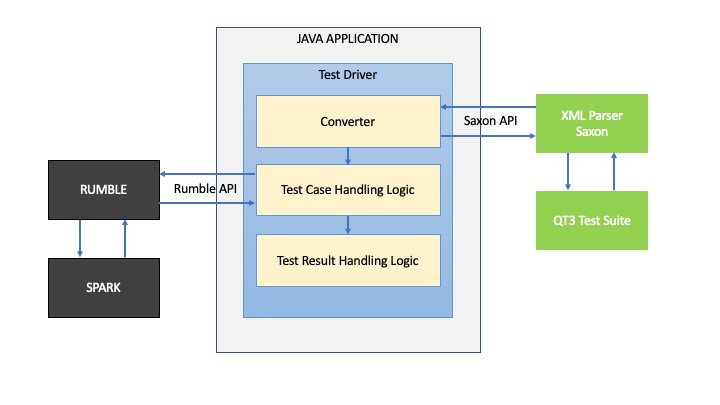
\includegraphics[width=\linewidth]{architecture_diagram_phase_2.jpg}
	\vspace*{-15mm}
	\caption{Phase 1 Architecture Overview}
	\label{fig:Phase2_Architecture}
\end{figure}

\subsection{Results}
As we have seen in Section \ref{Phase2_Converter}, Crashes were not only capturing tests that are not JSONiq and needed conversion. They were also including the tests that could not succeed simply because Rumble does not support that feature, type or error code. In Table \ref{tab:Phase2_Supported Types} we can see the limited amount of supported types and error codes compared to XQuery w3 specification for which we are able to verify assertion. All others would then be ignored and classified differently. Furthermore, some of them were introducing dependencies. For example, in dependency tag it was possible to have request for particular version of XPath, XQuery or XSLT. While Rumble is backwards compatible with all versions of XPath and XQuery, it does not support XSLT. We have therefore created and divided test cases into 7 groups:
\begin{enumerate}
	\item Success – Test that is passing the assertion and does not need Converter
	\item Managed – Tests that would have failed assertion, but they were modified with hard-coded conversion into JSONiq using Converter
	\item Skipped – Test that is not JSONiq and thus expectedly fails assertion. These tests should not be converted to JSONiq
	\item Failed – Tests that are failing because there is a bug in Rumble API or Test Driver implementation. 
	\item Dependency – Tests that are failing because dependency is not supported
	\item Unsupported – Tests that are failing because type, feature or error code is not supported yet
	\item Crash – Any other exception
\end{enumerate}

After introduction of the 7 above mentioned cases, together with small adjustments and bug changes, we were able to obtain:
\begin{table}[h!]
	\centering
	\begin{tabular}{|l|r|r|}
		\hline
		\multicolumn{1}{|c|}{Scenario} & \multicolumn{1}{c|}{Total test-cases} & \multicolumn{1}{c|}{\% of all test-cases} \\ \hline
		Success                        & 2686                                  & 8.52                                      \\ \hline
		Managed                        & 4211                                  & 13.36                                     \\ \hline
		Fail                           & 2554                                  & 8.10                                      \\ \hline
		Skipped                        & 5                                     & 0.02                                      \\ \hline
		Dependency                     & 1481                                  & 4.70                                      \\ \hline
		Crash                          & 13171                                 & 41.79                                     \\ \hline
		Unsupported                    & 7412                                  & 23.52                                     \\ \hline
	\end{tabular}
	\caption{Phase 2 Results Overview}
	\label{tab:Phase2_ResultTable}
\end{table}

Managed category was introduced as it was identified that with simple hard-coded conversion we are able to obtain around 4200 passed tests increasing total percentage of passed tests by roughly 12\%. At first, it seems that Success and Managed should be grouped into single category, but we decided to keep them separated. The reason behind is that while fixing bugs in both Rumble and Test Driver, we will increase the number of Success test cases. At the same time, we want to keep the track of Managed ones, because in Phase 3 Implementation we are planning to generalize the hard-coded conversion and create pure JSONiq Test Suite based on given XML ones.

For Skipped tests, these are the ones that it would not make sense to try to convert them to JSONiq. One example is XSLT tests and those should be skipped. We are keeping them in separate list as in Phase 3 Implementation we will skip from output and not include them in pure JSONiq Test Suite.

The main goal of performing iterations was to go through all the crashes and try to completely eliminate them. By doing so we would also improve the statistics by classifying them into other categories. At the same time, we were manually investigating test cases and trying to find the root cause. For some of them, our Test Driver implementation was improved. For some it was identified that the XQuery function was not yet supported by Rumle or it was having bugs so Rumble implementation was also improved. List of dependencies that were found in Test Suite were documented and classified according to Rumble documentation. The list is presented in Table \ref{tab:Phase2_DependencyList} \todo{maybe some reference here, ask Fourny}. 

Final goal was to identify test-cases that fail but can be converted to JSONiq. They could not be included into the automatic distinction of 7 above mentioned cases and had to be handled manually. They also helped with identifying what Phase 3 conversion also had to support.

\begin{table}[]
	\begin{tabular}{ll}
		\textbf{Dependency name}           & \textbf{Status}              \\
		higherOrderFunctions               & supported                    \\
		moduleImport                       & supported                    \\
		arbitraryPrecisionDecimal          & supported                    \\
		schemaValidation                   & not supported (XML specific) \\
		schemaImport                       & not supported (XML specific) \\
		advanced-uca-fallback              & not supported                \\
		non\_empty\_sequence\_collection   & not supported yet            \\
		collection-stability               & not supported yet            \\
		directory-as-collection-uri        & not supported yet            \\
		non\_unicode\_codepoint\_collation & not supported                \\
		staticTyping                       & not supported yet            \\
		simple-uca-fallback                & not supported                \\
		olson-timezone                     & not supported yet            \\
		fn-format-integer-CLDR             & not supported yet            \\
		xpath-1.0-compatibility            & not supported (XML specific) \\
		fn-load-xquery-module              & not supported yet            \\
		fn-transform-XSLT                  & not supported yet            \\
		namespace-axis                     & not supported (XML specific) \\
		infoset-dtd                        & not supported (XML specific) \\
		serialization                      & not supported yet            \\
		fn-transform-XSLT30                & not supported yet            \\
		remote\_http                       & not supported                \\
		typedData                          & not supported                \\
		schema-location-hint               & not supported (XML specific) \\
		calendar                           & not supported yet            \\
		unicode-version                    & supported                    \\
		unicode-normalization-form         & supported                    \\
		format-integer-sequence            & not supported yet            \\
		xsd-version                        & supported                    \\
		xml-version                        & supported                    \\
		default-language                   & only "en" supported          \\
		language                           & only "en" supported          \\
		spec                               & only "XT30+" not supported   \\
		limits                             & not supported yet           
	\end{tabular}
	\caption{Supported Dependency List }
	\label{tab:Phase2_DependencyList}
\end{table}

\section{Phase 3 implementation}
\todo{ Emphasize that for Converter itself we need a plugin architecture and draw it. So that you can include and exclude some conversion. }
\subsection{Description}
\label{Phase3_Description}
The main issue of Converter described in Section \ref{Phase2_Converter} was that it was hard-coded conversion using Java String.replace method. Such implementation can be very unstable. For example, we can look at 5th item of "other conversions" mentioned in Section \ref{Phase2_Converter} - replacing ' with ". For example, test-case Literals009 is verifying whether "test' is a valid String Literal. With our hard-coded conversion, we will make this test-case valid String Literal instead of it causing an Error Code XPST0003. Therefore, we have decided to implement Test Converter as separate module. It's main purpose is to generalize the hard-coded conversion. It would take QT3TS as Input and generate pure JSONiq Test Suite as output.

For implementing Test Converter we decided to create following classification of test-cases:
\begin{enumerate}
	\item Fails, as expected and should not be converted to JSONiq. It will never be supported
	\item Fails, as expected since it is not supported yet
	\item Fails, but can be rescued with simple conversion. Any simple conversion like removing the "fn" prefix 
	\item Fails, but can be converted to JSONiq. Any complicated conversion like XML to JSON
	\item Fails, because it is bug in Rumble
	\item Succeeds
\end{enumerate}

With this classification, we want to reuse most of Phase 2 Implementation Results presented in Table \ref{tab:Phase2_ResultTable}.

If we compare above described classification with classification in Table \ref{tab:Phase2_ResultTable}, we can notice that Fail corresponds to Item 5. Item 6 corresponds to Success. Managed corresponds to Item 3. Item 2 corresponds to Unsupported and Dependency. Skipped correspond to Item 1. 

Performing iterations in Phase 1, we want to distribute all Crashes into some of Item 4 or 1. Of course, it is in our interest to identify as many test-cases as possible as Item 4 and perform conversion in Test Converter. Everything that we cannot convert, we will classify as Item 1. 

Items 1 and 2 will be excluded from Test Converter output. However, we also need to take into account that over time, as Rumble implementation improves, tests from Item 1 will be distributed into 4 other categories. Therefore, we want to make highly modular and extensible architecture. We have decided to maintain a list of conversions that need to be performed. This list will be compiled by using all results obtained so far. The architecture with work as a "plugin". It will allow us to specify what conversions we will perform and what we will include or exclude from output. The important design decision remaining is the Data Format of the Test Converted output.

\subsubsection{JSONiq and Test Converter Data Format}
The JSONiq extension to XQuery allows processing XML and JSON natively and with a single language. This extension is based on the same data model as the core JSONiq and is based on the same logical concepts. Because of the complexity of the XQuery grammar, the JSONiq extension to XQuery has a less pleasant syntax that the JSONiq core. \todo{maybe cite something}. When designing the Test Converter, we could have decided to use either XML or JSON as the under-laying language. However, as our Test Driver was already implemented in the previous phase and was expecting XML as input and using the before mentioned Saxon for parsing it, we have decided to keep the same language for output of the Test Converter. 

\subsection{Architecture}
The overview of scenario described in \ref{Phase3_Description} can be seen in Figure \ref{fig:Phase3_Architecture}
\begin{figure}[h!]
	\vspace*{-5mm}
	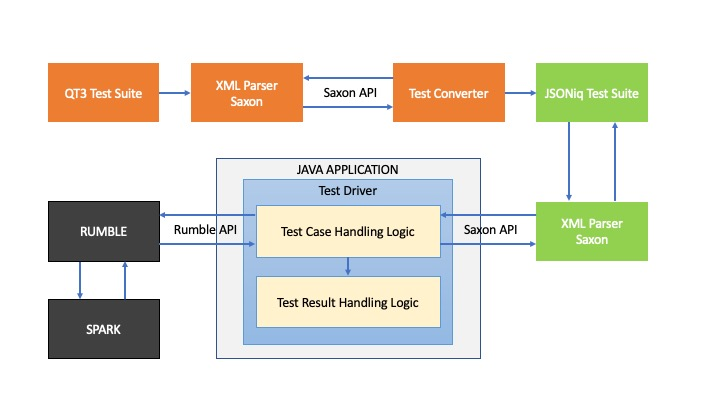
\includegraphics[width=\linewidth]{architecture_diagram_phase_3.jpg}
	\vspace*{-15mm}
	\caption{Phase 1 Architecture Overview}
	\label{fig:Phase3_Architecture}
\end{figure}